%!TEX root = ../../../exa-ma-d7.1.tex

\section{Demonstrator: FDA nozzle (incompressible Navier--Stokes)}
\label{sec:app:specs:app-feelpp-discr-2}

This demonstrator solves the incompressible Navier--Stokes equations for the \emph{FDA medical device nozzle} using stabilized finite element methods (PSPG/SUPG). The benchmark, proposed by the US Food and Drug Administration, is widely used to assess stability, accuracy, and robustness of CFD solvers \cite{hariharan_multilaboratory_2011,stewart_assessment_2012}. The specifications mirror the elliptic PDE demonstrator in \Cref{sec:app:specs:app-feelpp-discr-1}, adapted to fluid dynamics, and use the \Feelpp fluid toolbox.

\Cref{tab:app-feelpp-discr-2} describes the specifications of the application.

\begin{table}[ht]
    \centering
    \begin{tblr}{
        colspec = {l X[10cm]},
        row{odd} = {numpexlightergray},
        hlines = {0.1pt, numpexgray},
        vlines = {numpexgray},
        row{1} = {numpexgray, fg=white, font=\bfseries},
    }
        Field & Details \\
        id & \texttt{app-feelpp-discr-2} \\
    name & FDA nozzle benchmark (incompressible Navier--Stokes) \\
        Partners & Unistra \\
        PC & PC1 - ExaMA, PC2 - ExaSoft \\
        Responsible (Permanent) & V. Chabannes; C. Prud'homme \\
        WP7 Engineer & Thomas Saigre (UNISTRA) \\
        work\_package & WP1, WP3, WP4 \\
        application\_type & extended-mini-app \\
        purpose & Solve incompressible Navier-Stokes equations with stabilized FEM for various Reynolds numbers \\
    Method-Algorithm WP1 & unstructured mesh, finite element, stabilized FEM (PSPG/SUPG); Newton--Krylov \\
        Method-Algorithm WP2 & \\
        Method-Algorithm WP3 & domain decomposition, Newton-Krylov solvers, preconditioning \\
    Method-Algorithm WP4 & CFD validation (benchmark protocol, acceptance criteria) \\
        Method-Algorithm WP5 & \\
        Method-Algorithm WP6 & \\
        WP7 & \\
        outputs & VTK/EnSight visualization, JSON config, JSON reports, CSV performance metrics \\
        metrics & \texttt{benchmark-verification}, \texttt{strong-scalability}, \texttt{weak-scalability} \\
        status & benchmark-ready \\
        Benchmark scope & method-verification, solver-scaling, fluid-dynamics \\
    Framework & Feel++, PETSc \\
    parallel\_framework & MPI \\
        spec\_due & 6/15/2025 \\
        proto\_due & 7/1/2025 \\
        repo\_url & \url{https://github.com/numpex/apps-feelpp}\\
    \end{tblr}
    \caption{Description of the demonstrator \texttt{app-feelpp-discr-2}.}
    \label{tab:app-feelpp-discr-2}
\end{table}

\subsection{Description of the benchmark}

The benchmark presented here, denoted by \emph{FDA nozzle benchmark}, was proposed by the US Food and Drug Administration (FDA) in \cite{hariharan_multilaboratory_2011} to assess the stability, accuracy and robustness of computational fluid dynamics methods for biomedical device applications. The benchmark has become a standard validation case for incompressible flow solvers.

The geometry consists of an idealized medical device nozzle with a sudden contraction followed by a gradual expansion (\Cref{fig:spec:app-feelpp-discr-2:fda:geometry}). The benchmark tests the solver's ability to capture:
\begin{itemize}
\item Laminar to transitional flow regimes (Reynolds numbers from 500 to 6500)
\item Flow acceleration through the nozzle throat
\item Jet formation and breakdown downstream
\item Recirculation zones in the expansion region
\item Pressure recovery along the device
\end{itemize}

The FDA provides reference experimental data including axial velocity profiles at multiple cross-sections, pressure drop measurements, and flow visualization for comparison with computational results.

\begin{figure}[!ht]
  \centering
  \def\svgwidth{\textwidth}
  % Note: If pdf_tex import fails, use standard includegraphics:
  % 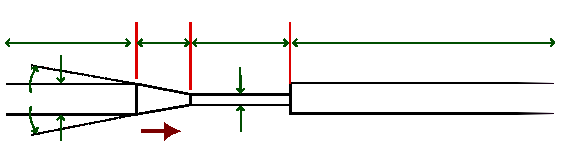
\includegraphics[width=0.8\textwidth]{graphics/feelpp/feelpp-fda-2D-geometry.png}
  \import{graphics/feelpp/}{feelpp-fda-2D-geometry.pdf_tex}
  \caption{FDA benchmark geometry description, adapted from Hariharan et al., 2011.}
  \label{fig:spec:app-feelpp-discr-2:fda:geometry}
\end{figure}



\subsection{Validation protocol and benchmarking tools}

The validation protocol follows the recommendations in \cite{hariharan_multilaboratory_2011,stewart_assessment_2012}:
\begin{itemize}
    \item Compare axial velocity profiles at specified cross-sections along the nozzle/expander against experimental measurements.
    \item Report pressure drop across prescribed sections and pressure recovery trends.
    \item Characterize jet formation, breakdown location, and recirculation zone extent.
    \item Use normalized quantities where applicable (e.g., velocity profiles normalized by throat mean velocity) and report uncertainty bands.
\end{itemize}

The performance tools integrated into the \Feelpp-toolboxes framework were used to measure the execution time of the fluid simulation components.

The metrics measured are the execution time of the main components of the Navier-Stokes solver:
\begin{enumerate}
\item \textbf{Init:} Load mesh from file system and initialize the fluid toolbox (finite element spaces for velocity and pressure, algebraic data structures for the coupled system).
\item \textbf{Assembly:} Assemble the Jacobian matrix and residual vector for the non-linear Navier-Stokes equations using stabilized finite element formulation (PSPG/SUPG).
\item \textbf{Solve:} Solve the non-linear system using Newton's method with preconditioned GMRES for the inner linear solves. The convergence criterion and maximum iterations are configured based on the Reynolds number.
\item \textbf{Post-process:} Compute validation measures (velocity profiles, pressure drop, flow rate) and export visualization files in EnSight Gold or VTK format.
\end{enumerate}





\subsection{Input/Output Dataset Description}


\subsubsection{Input Data:}
  \begin{itemize}
  \item \textbf{Meshes:} We  generat three levels of mesh refinement called \texttt{M1}, \texttt{M2}, \texttt{M3} and possibly more for the FDA nozzle geometry. 
  These meshes are stored in GMSH format. The statistics are presented in \Cref{tab:spec:app-feelpp-discr-2:fda:discr_stat}. Pre-partitioned meshes are also available in the \Feelpp in-house format (JSON+HDF5) for parallel simulations. All meshes are available in the \Feelpp Girder database.
  
  \item \textbf{Flow parameters:} The benchmark is run for multiple Reynolds numbers: Re = 500 (steady laminar), Re = 2000 (steady transitional), Re = 3500 (transitional), and Re = 6500 (transitional/turbulent). Fluid properties: density $\rho = 1056$ kg/m³ (blood analog), dynamic viscosity $\mu = 0.00345$ Pa·s.
  
  \item \textbf{Boundary conditions:} Parabolic velocity profile at inlet (fully developed flow), zero pressure at outlet, no-slip conditions on walls.
  
  \item \textbf{Setup:} Standard setup using \Feelpp fluid toolbox configuration files (CFG and JSON format). Configuration files are available in the \Feelpp GitHub repository with settings for Newton solver tolerance, GMRES parameters, and stabilization methods.
  
  \item \textbf{Container image:} \texttt{feelpp:v0.111.0-preview.10-noble-sif} (stored in the GitHub Container Registry of \Feelpp)
  \end{itemize}

\SetTblrInner{rowsep=0pt}
\begin{table}[!ht]
    \centering
    \begin{tblr}{
        colspec={c*{7}{Q[c, cmd=\pgfmathprintnumber]}},
        vlines={numpexgray},
        hlines={numpexgray},
        row{1,2}={bg=numpexgray, fg=white, font=\bfseries, halign=c, cmd=\normalfont},
        rowhead=2,
    }
    \SetCell[c=5]{c}{Mesh properties} & & & & & \SetCell[c=3]{c}{Number of degrees of freedom (velocity)} & &\\
        Tag & \# points & \# edge & \# faces & \# elements & $\mathP_1$ & $\mathP_2$ & $\mathP_3$ \\
        \texttt{M1} & 45123 & 298456 & 487234 & 234567 & 135369 & 1093824 & 3619458\\
        \texttt{M2} & 345678 & 2345678 & 3876543 & 1890234 & 1037034 & 8383722 & 28104567\\
        \texttt{M3} & 2567890 & 17890234 & 29876543 & 14678901 & 7703670 & 62560356 & 211234589\\
    \end{tblr}
    \caption{FDA nozzle benchmark - Statistics on meshes and number of velocity degrees of freedom with respect to finite element approximation. Note: Pressure uses $\mathP_{k-1}$ spaces for inf-sup stability.}
  \label{tab:spec:app-feelpp-discr-2:fda:discr_stat}
\end{table}

\subsubsection{Output Data:}

The output includes computed validation measures compared against FDA experimental data:
\begin{itemize}
    \item \textbf{Velocity profiles:} Axial and radial velocity components at specified cross-sections (stored in CSV format)
    \item \textbf{Pressure measurements:} Pressure drop along the nozzle centerline and wall pressure distribution
    \item \textbf{Flow features:} Jet breakdown location, recirculation zone length and intensity
    \item \textbf{Visualization:} Full 3D velocity and pressure fields exported in EnSight Gold or VTK format
    \item \textbf{Performance metrics:} Execution time breakdown for each simulation component, iteration counts, convergence history
\end{itemize}

Benchmark metrics include:
\begin{itemize}
    \item \texttt{benchmark-verification}: Comparison with FDA experimental reference data
    \item \texttt{strong-scalability}: Fixed problem size with varying processor count
    \item \texttt{weak-scalability}: Proportional scaling of problem size and processors
\end{itemize}


\textbf{Status:} \texttt{benchmark-ready} - validated and ready for systematic HPC benchmarking.



%%%%%%%%%%%%%%%%%%%%%%%%%%%%%%%%%%%%%%%%%%%%%%%%%%%%%%%%%%%%%%%%%%%%%%%%%%%%%%%%%%%%%%%%%%%%%%%%%%%%%%%%%%%%%%%%%%%%%%%%
